%!TEX root = /Users/jakubkonka/Thesis/Thesis.tex
\chapter{Simulation Model of the Digital Marketplace}
\label{cha:simulation_model_of_the_digital_marketplace}

\minitoc
\vspace{10mm}

\section{Description of the Model}
\label{sec:description_of_the_model_dmappendix}

\subsection{High-level Overview}
\label{sub:high_level_overview_dmappendix}
The DMP is modeled using the object-oriented paradigm. The entities involved in the DMP are represented by Bidder and DMEventHandler classes. The Bidder class stores attributes specific to a network operator such as costs per service type. The DMEventHandler class, on the other hand, generates subscribers and service requests, runs auctions, etc. Both classes are described in more detail in the next two sections.

When the simulation is running, two types of events are generated: \lstinline{SR_EVENT} and \lstinline{ST_EVENT} (Figure~\ref{fig:dm_events_dmappendix}). \lstinline{SR_EVENT} signifies a new service request by a subscriber, and triggers an auction between the network operators; \lstinline{ST_EVENT} signifies that a subscriber has finished using a wireless service, and the servicing network operator can recover any resources dedicated to that subscriber, such as the bit-rate required by the service.
\begin{figure}[t]
	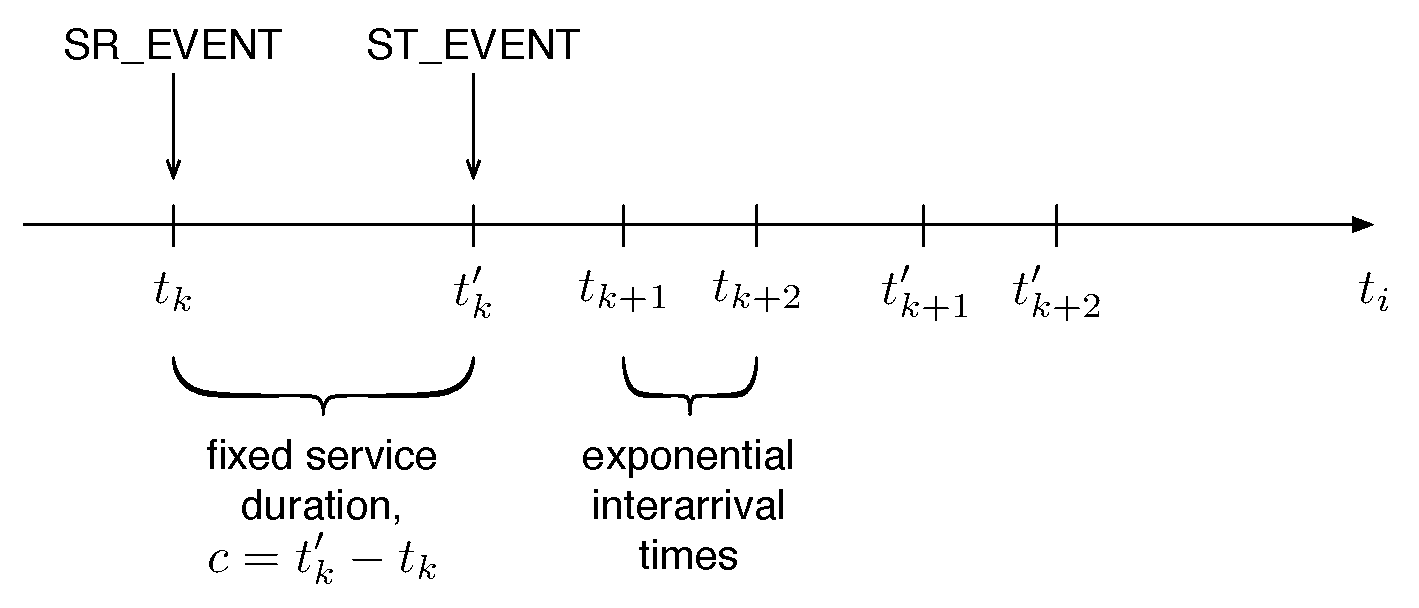
\includegraphics[width=\figsize]{Appendices/Figures/dm_events}
	\caption{Events generated during the simulation of the DMP}
	\label{fig:dm_events_dmappendix}
\end{figure}
If we let $t_k$ for all $k\in I$ denote the arrival time of service request $s_k$, then $t_k$ corresponds to the arrival time of an \lstinline{SR_EVENT}. Furthermore, every \lstinline{SR_EVENT} has a corresponding \lstinline{ST_EVENT} such that the time difference between the two is constant; that is, if the arrival time of \lstinline{ST_EVENT} is $t_k'$, then $c = t_k - t_k'$ for all $k\in I$. The time difference $c$ represents the duration of a wireless service requested by a subscriber, and currently, it is assumed to be $c=2.5$ minutes. The interarrival rate of \lstinline{SR_EVENT}s, on the other hand, is currently assumed to be exponentially distributed with parameter $\lambda=1$ service request per second. Since it is difficult to quantify the distribution of the duration of wireless services, it is assumed that the duration is constant in order to keep the model as simple as possible, while, at the same time, the minimum amount of stochasticity is achieved through the exponentially drawn interarrival times of service requests.

In the course of the simulation, the following performance measures are gathered for analysis:
\begin{itemize}
	\item the reputation rating history for each network operator---an indicator of the credibility of network operators over time.
	\item the number of secured auctions (or service requests) by each network operator---an indicator of the market share between network operators over time.
\end{itemize}

It is further assumed that there are two network operators competing in the DMP. This allows for the use of the equilibrium bidding strategy functions derived in Chapter~\ref{cha:network_selection_mechanism_in_the_digital_marketplace}. The subscribers (and  hence, the price weights and service types) are pseudo-randomly generated.

\subsection{Bidder Class}
\label{sub:bidder_class_dmappendix}
As mentioned in the High-level Overview section, the Bidder class is tasked with the representation of a network operator. It implements attributes such as costs, current reputation rating, total bit-rate, currently available bit-rate, and subscriber success report list (Figure~\ref{fig:bidder_class_dmappendix}). The class also implements the bidding behavior of a network operator, and reputation rating update algorithm. Furthermore, the Bidder class populates subscriber success report list, and updates the currently available bit-rate of a network operator.

\begin{figure}[t]
	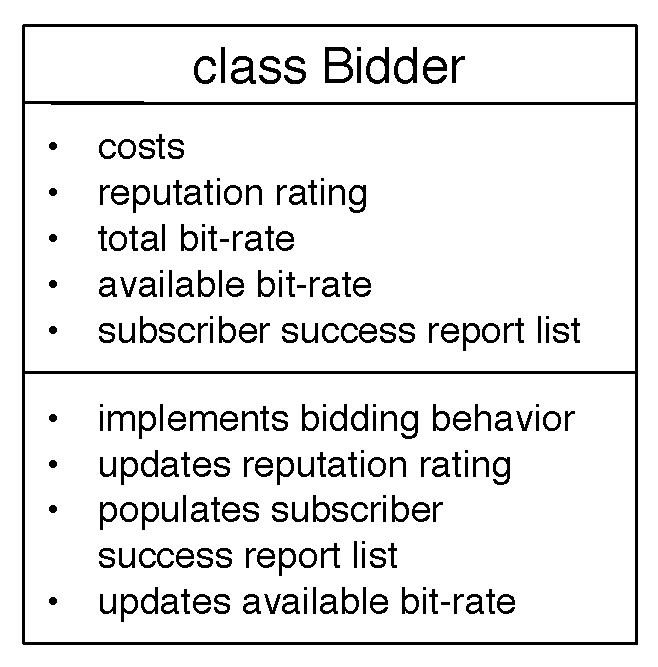
\includegraphics[width=2in]{Appendices/Figures/bidder_class}
	\caption{Bidder class}
	\label{fig:bidder_class_dmappendix}
\end{figure}

It is assumed that costs do not change over time, but differ only per service type. Therefore, the cost of web-browsing service might be different from an e-mail service, but neither will change in the course of the simulation. Furthermore, the costs per service type may be specified manually before the simulation executes, or pseudo-randomly drawn from a uniform distribution over the discretized interval $[0,1]$ by the simulation software otherwise.

Initially, the reputation rating is set to $0.5$ for all network operators as discussed in Section~\ref{sec:mathematical_description_dynamic}. Afterwards, for each secured service request by a network operator, the reputation rating is updated according to Equation~\eqref{eq:def_rep_update_lebodic_dynamic}. If a network operator does not secure a service request, then their reputation rating remains constant at that instance of time. For example, if network operator $j$ does not secure a service request at time $t_k$, then $r^j_k = r^j_{k-1}$.

The total available bit-rate has to be manually specified before each simulation for all network operators. The currently available bit-rate, on the other hand, is updated automatically as the simulation progresses. Initially, it equals the total available bit-rate. Then, as a network operator secures service requests, it is decreased by an amount equal to the required bit-rate of the service request for the duration of that service; that is, if network operator $j$ secures service request $s_k$ at time $t_k$, then for $c=2.5$ minutes and provided $t_{k+1}-t_k\le c$, their available bit-rate becomes
\begin{equation*}
	z^j_{k+1} =
	\left\{
	\begin{array}{ll}
		z^j_k - s^{bw}_k &\text{if } z^j_k - s^{bw}_k\ge 0, \\
		0 &\text{otherwise}.
	\end{array}
	\right.
\end{equation*}

The subscriber success report list is updated automatically as the simulation progresses according to Equation~\eqref{eq:def_users_satisfaction_bandwidth_dynamic}. Therefore, if the available bit-rate of the network operator exceeds the required bit-rate of the service, the subscriber is satisfied, and $\sigma_k^j = 1$ is stored in the subscriber success report list. Otherwise, $\sigma_k^j = 0$ is stored.

The Bidder class, by default, assumes that network operators bid myopically; that is, they treat each auction as a one-shot event, and hence, they neglect past as well as future interactions with the other network operators. Although in reality they are likely to bid in a more sophisticated fashion, it is a valid starting point especially in the case of two competing network operators since the analytical solution to a problem of two competing network operators in a one-shot DMP auction exists (see Section~\ref{sec:indirect_approach_static}, Chapter~\ref{cha:network_selection_mechanism_in_the_digital_marketplace}). 

The Bidder and the DMEventHandler classes interface according to the following sequence:
\begin{enumerate}
	\item \lstinline{SR_EVENT} (and hence, service request with all the relevant parameters) is generated;
	\item DMEventHandler class calls for an auction;
	\item an object of Bidder type (and hence, network operators) submit their bids according to the implemented bidding behavior;
	\item DMEventHandler class elects the winner of the auction;
	\item \lstinline{ST_EVENT} is generated for the winner;
	\item reputation rating, available bit-rate, and subscriber success report list are updated accordingly.
\end{enumerate}

\subsection{DMEventHandler Class}
\label{sub:dmeventhandler_class_dmappendix}
\lstinline{SR_EVENT} exponential interarrival times; \lstinline{ST_EVENT} is scheduled after each \lstinline{SR_EVENT} at a constant interval of 2.5 minutes. Stores possible service request types such as \lstinline{WEB_BROWSING} and \lstinline{EMAIL} with their required bit-rates. Currently, it is assumed that \lstinline{WEB_BROWSING} requires 512 kbps, while \lstinline{EMAIL} requires 256 kbps. DMEventHandler also runs auctions and elects the winner. FIX:ME \cite{DMKonkaIaria12}

\begin{figure}[t]
	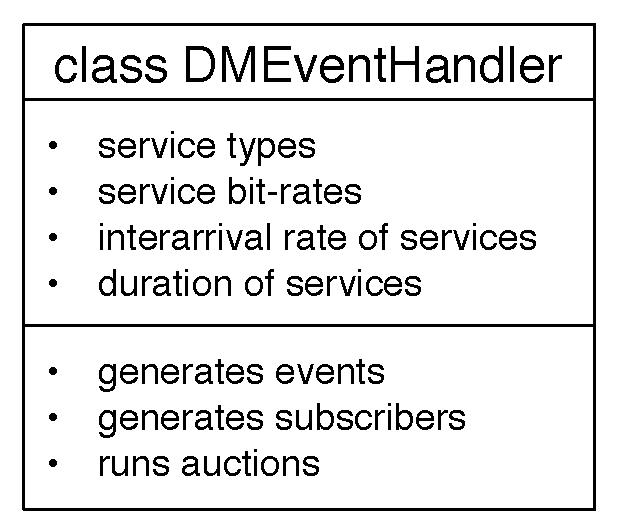
\includegraphics[width=2in]{Appendices/Figures/dmeventhandler_class}
	\caption{DMEventHandler class}
	\label{fig:dmeventhandler_class_dmappendix}
\end{figure}

